% ========================================= TEMPLATE INFO ========================================
%
% Author:       P4ntomime
% Version:      1.0.0
% Last updated: 2024-02-18
% Brief:        A LaTeX template for summaries. See README.md for more information.
% 
% ================================================================================================
\documentclass[8pt, a4paper, twoside]{extarticle}
% Font size:    8pt
% Paper size:   A4
% style:        twoside (needed, so odd and even pages have different margins)
% orientation:  portrait. (use 'landscape' for landscape orientation)


% ========================================= DOCUMENT INFO =========================================
\def\title{Energiesysteme}           % title
\def\shorttitle{EnSys} % short title (displayed as PDF title)
\def\dozent{Dr. A Fuchs, Dr. T Demiray}         % lecturer
\def\semester{6. Semester}     % semester
\def\author{Luca Loop}        % author(s)
\def\repo{https://github.com/Luca-ET/EnSys.git}             % repository link
\def\version{1.0.\today}    % version
\def\pagelimit{100}           % page limit -> causes pages after limit to be red
\def\titleoption{compact}   % options: ultra compact, compact, normal
\def\enableToC{true}

% ================================= PACKAGES, SETUP AND COMMANDS ==================================
\input{preamble.tex}


% =========================================== DOCUMENT ============================================
\begin{document}
    \begin{layout}
        %\section{Energie- und Elektrizitätswirtschaft}

\subsection{Masseinheiten}

\begin{tabular}{|l|c|l|}
    \hline
    \textbf{Masseinheit}    & \textbf{Zeichen}  & \textbf{Umrechnung} \\
    \hline
    Watt                    & (W)               & \\ 
    Pferdestärke            & (PS)              & 1 PS $\approx$ 735 W \\ 
    \hline
    Joule                   & (J)               & \\ 
    Wattsekunde             & (Ws)              & 1 Ws = 1 J \\ 
    Kilowattstunde          & (kWh)             & 1 kWh = 3 600 000 J = 3,6 MJ \\ 
    Kalorie                 & (cal)             & 1 cal$_{IT}$ = 4,1868 J \\ 
    \hline
\end{tabular}


\subsection{Umrechnungsfaktoren}

\begin{tabular}{|l|c|c|c|c|}
    \hline
    \textbf{\textbf{Von | Zu}}  & \textbf{J = Ws}           & \textbf{kWh}                  & \textbf{GWh}              & \textbf{cal} \\
    \hline
            J = Ws              & 1                         & $0,2778 \cdot 10^{-6}$        & $0,2778 \cdot 10^{-12}$   & 0,2388 \\
            TJ                  & $1 \cdot 10^{12}$         & $0,2778 \cdot 10^{6}$         & 0,2778                    & $0,2388 \cdot 10^{12}$ \\
            kWh                 & $3,6 \cdot 10^{6}$        & 1                             & $1 \cdot 10^{-6}$         & $0,8598 \cdot 10^{6}$ \\
            GWh                 & $3,6 \cdot 10^{12}$       & $1 \cdot 10^{6}$              & 1                         & $0,8598 \cdot 10^{12}$ \\
            cal                 & 4,1868                    & $1,163 \cdot 10^{-6}$         & $1,163 \cdot 10^{-12}$    & 1 \\
    \hline
\end{tabular}


\subsection{Dezimalfaktoren}
\begin{tabular}{|l|c|r|}
    \hline
    \textbf{Bezeichnung}    & \textbf{Faktor}   & \textbf{Wert} \\
    \hline
    Kilo  (k)               & \(10^3\)          & 1 000 \\
    Mega  (M)               & \(10^6\)          & 1 000 000 \\
    Giga  (G)               & \(10^9\)          & 1 000 000 000 \\
    Tera  (T)               & \(10^{12}\)       & 1 000 000 000 000 \\
    Peta  (P)               & \(10^{15}\)       & 1 000 000 000 000 000 \\
    \hline
\end{tabular}


\subsection{Energien}

\subsubsection{Potentielle Energie $W_{\text{pot}}$}
$\boxed{W_{\text{pot}} = m \cdot g \cdot h}$ \quad $g = 9.81 \frac{m}{s^2}$

\renewcommand{\arraystretch}{1.2} % Erhöht Zeilenhöhe für bessere Lesbarkeit
\begin{tabular}{@{} l p {4cm} l @{}}
    $[W_{\text{pot}}]$  & Potentielle Energie   \dotfill & $Ws = Nm = J$ \\
    $[m]$               & Masse                 \dotfill & $kg$ \\
    $[g]$               & Erdbeschleunigung     \dotfill & $\frac{m}{s^2}$ \\
    $[h]$               & Höhenunterschied      \dotfill & $m$ \\
\end{tabular}

\subsubsection{Kinetsche Energie $W_{\text{kin}}$}
$\boxed{W_{\text{kin}} = \frac{1}{2} \cdot m \cdot v^2}$

\renewcommand{\arraystretch}{1.2} % Erhöht Zeilenhöhe für bessere Lesbarkeit
\begin{tabular}{@{} l p {4cm} l @{}}
    $[W_{\text{kin}}]$  & Kinetische Energie   \dotfill & $Ws = Nm = J$ \\
    $[m]$               & Masse                \dotfill & $kg$ \\
    $[v]$               & Geschwindigkeit      \dotfill & $m/s$ \\
\end{tabular}


\subsubsection{Feder Energie $W_{\text{F}}$}
$\boxed{W_{\text{F}} = \frac{1}{2} \cdot F \cdot s}$

\renewcommand{\arraystretch}{1.2} % Erhöht Zeilenhöhe für bessere Lesbarkeit
\begin{tabular}{@{} l p {4cm} l @{}}
    $[W_{\text{F}}]$  & Federenergie                \dotfill & $Ws = Nm = J$ \\
    $[F]$             & Kraft                       \dotfill & $N = kg \cdot m/s^2$ \\
    $[s]$             & Verschiebung (Auslenkung)   \dotfill & $m$ \\
\end{tabular}


\subsubsection{Kondensator Energie $W_{\text{C}}$}
$\boxed{W_{\text{C}} = \frac{1}{2} \cdot C \cdot U^2}$

\renewcommand{\arraystretch}{1.2} % Erhöht Zeilenhöhe für bessere Lesbarkeit
\begin{tabular}{@{} l p {4cm} l @{}}
    $[W_{\text{C}}]$  & Kondensatorenergie    \dotfill & $Ws = Nm = J$ \\
    $[C]$             & Kapazität             \dotfill & $F = \frac{As}{V}$ \\
    $[U]$             & Spannung              \dotfill & $V$ \\
\end{tabular}


\subsubsection{Induktivität Energie $W_{\text{L}}$}
$\boxed{W_{\text{L}} = \frac{1}{2} \cdot L \cdot I^2}$

\renewcommand{\arraystretch}{1.2} % Erhöht Zeilenhöhe für bessere Lesbarkeit
\begin{tabular}{@{} l p {4cm} l @{}}
    $[W_{\text{L}}]$  & Induktivitätsenergie  \dotfill & $Ws = Nm = J$ \\
    $[L]$             & Induktivität          \dotfill & $H = \frac{Vs}{A}$ \\
    $[I]$             & Stromstärke           \dotfill & $A$ \\
\end{tabular}


\subsubsection{Batterie Energie $W_{\text{bat}}$}
$\boxed{W_{\text{bat}} = Q \cdot U}$

\renewcommand{\arraystretch}{1.2} % Erhöht Zeilenhöhe für bessere Lesbarkeit
\begin{tabular}{@{} l p {4cm} l @{}}
    $[W_{\text{bat}}]$  & Batterieenergie       \dotfill & $Ws = Nm = J$ \\
    $[Q]$               & Elektrische Ladung    \dotfill & $C = As$ \\
    $[U]$               & Spannung              \dotfill & $V$ \\
\end{tabular}


\subsubsection{Thermische Energie $W_{\text{th}}$}
$\boxed{W_{\text{th}} = m \cdot c \cdot (\vartheta_1 - \vartheta_2)}$ \quad $c_{Wasser} = 4187 \frac{J}{kg \cdot K}$

\renewcommand{\arraystretch}{1.2} % Erhöht Zeilenhöhe für bessere Lesbarkeit
\begin{tabular}{@{} l p {4cm} l @{}}
    $[W_{\text{th}}]$       & Thermische Energie          \dotfill & $Ws = Nm = J$ \\
    $[m]$                   & Masse                       \dotfill & $kg$ \\
    $[c]$                   & Spezifische Wärmekapazität  \dotfill & $\frac{J}{kg \cdot K}$ \\
    $[\vartheta_1]$         & Anfangstemperatur           \dotfill & $^\circ C$ oder $K$ \\
    $[\vartheta_2]$         & Endtemperatur               \dotfill & $^\circ C$ oder $K$ \\
\end{tabular}



\subsubsection{Spezifische Energie $e$}

$\boxed{e = \frac{W}{m}}$ \quad $\boxed{W = e \cdot m}$

\renewcommand{\arraystretch}{1.2} % Erhöht Zeilenhöhe für bessere Lesbarkeit
\begin{tabular}{@{} l p {4cm} l @{}}
    $[e]$  & Spezifische Energie    \dotfill & $\frac{J}{kg}$ \\
    $[W]$  & Gesamtenergie          \dotfill & $J$ \\
    $[m]$  & Masse                  \dotfill & $kg$ \\
\end{tabular}


\subsubsection{Rotations Energie $W_{\text{rot}}$}
$\boxed{W_{\text{rot}} = \frac{1}{2} \cdot J \cdot \omega^2 }$ \quad $\boxed{W_{\text{rot}} = 2 \cdot J \cdot \pi^2 \cdot f^2 }$ \quad $\boxed{W_{\text{rot}} = \frac{J \cdot \pi^2 \cdot n^2}{1800}}$

$\boxed{\omega = 2 \cdot \pi \cdot f}$ \quad $\boxed{f = \frac{n}{60}}$ \quad $\boxed{n = f \cdot 60}$


\renewcommand{\arraystretch}{1.2} % Erhöht Zeilenhöhe für bessere Lesbarkeit
\begin{tabular}{@{} l p {5cm} l @{}}
    $[W_{\text{rot}}]$  & Rotationsenergie                      \dotfill & $Ws = Nm = J$ \\
    $[J]$               & Trägheitsmoment                       \dotfill & $kg \cdot m^2$ \\
    $[\omega]$          & Winkelgeschwindigkeit                 \dotfill & $\frac{rad}{s}$ \\
    $[f]$               & Drehfrequenz, Umdrehungen pro Sekunde \dotfill & $\frac{1}{s} = \frac{U}{\text{sek}}$ \\
    $[n]$               & Umdrehungen pro Minute                \dotfill & $\frac{1}{\text{min}} = \frac{U}{\text{min}}$ \\
\end{tabular}

\vspace{0.25cm}
\myul{\textbf{Massenträgheitsmoment $J$}}\\
\includegraphics[width=0.75\linewidth]{images/Physik_1-Mechanik.png}


\subsection{Leistung}

\subsubsection{Rotations Leistung $P_{rot}$}
$\boxed{P = M \cdot \omega}$ \quad $\boxed{P = M \cdot 2 \cdot \pi \cdot f }$ \quad $\boxed{P = \frac{M \cdot 2 \cdot \pi \cdot n}{60} }$

\renewcommand{\arraystretch}{1.2} % Erhöht Zeilenhöhe für bessere Lesbarkeit
\begin{tabular}{@{} l p {4cm} l @{}}
    $[P_{rot}]$ & Rotations Leistung        \dotfill & $W = \frac{J}{s} = \frac{Nm}{s}$ \\
    $[M]$       & Drehmoment                \dotfill & $Nm$ \\
    $[\omega]$  & Winkelgeschwindigkeit     \dotfill & $\frac{rad}{s}$ \\
    $[f]$       & Drehfrequenz              \dotfill & $Hz = \frac{1}{s}$ \\
    $[n]$       & Umdrehungen pro Minute    \dotfill & $\frac{1}{\text{min}} = \frac{U}{\text{min}}$ \\
\end{tabular}


\subsubsection{Thermische Leistung $P_{\text{th}}$}
$\boxed{P_{\text{th}} = \dot{m} \cdot c \cdot \Delta \vartheta}$ \quad $\boxed{\dot{m} = \rho \cdot \dot{V} }$

\renewcommand{\arraystretch}{1.2} % Erhöht Zeilenhöhe für bessere Lesbarkeit
\begin{tabular}{@{} l p {4cm} l @{}}
    $[P_{\text{th}}]$       & Thermische Leistung           \dotfill & $W = \frac{J}{s}$ \\
    $[\dot{m}]$             & Massenstrom                   \dotfill & $\frac{kg}{s}$ \\
    $[c]$                   & Spezifische Wärmekapazität    \dotfill & $\frac{J}{kg \cdot K}$ \\
    $[\Delta \vartheta]$    & Temperaturdifferenz           \dotfill & $K$ oder $^\circ C$ \\
    $[\rho]$                & Dichte                        \dotfill & $\frac{kg}{m^3}$ \\
    $[\dot{V}]$             & Volumenstrom                  \dotfill & $\frac{m^3}{s}$ \\
\end{tabular}


\subsubsection{Transmissions Wärmeverlustleistung $P_{VW}$}

$\boxed{P_{VW} = U \cdot A \cdot \Delta \vartheta}$

\renewcommand{\arraystretch}{1.2} % Erhöht Zeilenhöhe für bessere Lesbarkeit
\begin{tabular}{@{} l p {4cm} l @{}}
    $[P_{VW}]$              & Wärmeverlustleistung          \dotfill & $W = \frac{J}{s}$ \\
    $[U]$                   & Wärmedurchgangskoeffizient    \dotfill & $\frac{W}{m^2 \cdot K}$ \\
    $[A]$                   & Fläche                        \dotfill & $m^2$ \\
    $[\Delta \vartheta]$    & Temperaturdifferenz           \dotfill & $K$ \\
\end{tabular}


\subsubsection{Mechanische Leistung $P_{v}$}
$\boxed{P_v = F \cdot v}$ \quad $\boxed{F = m \cdot g}$

\renewcommand{\arraystretch}{1.2} % Erhöht Zeilenhöhe für bessere Lesbarkeit
\begin{tabular}{@{} l p {4cm} l @{}}
    $[P_v]$ & Mechanische Leistung   \dotfill & $W = \frac{J}{s} = Nm/s$ \\
    $[F]$   & Kraft                  \dotfill & $N = kg \cdot \frac{m}{s^2}$ \\
    $[m]$   & Masse                  \dotfill & $kg$ \\
    $[g]$   & Erdbeschleunigung      \dotfill & $\frac{m}{s^2}$ \\
    $[v]$   & Geschwindigkeit        \dotfill & $\frac{m}{s}$ \\
\end{tabular}


\subsubsection{Leistung der Solaranlage $P_{PV}$}
$\boxed{P_{PV} = \eta \cdot A \cdot E}$

\renewcommand{\arraystretch}{1.2} % Erhöht Zeilenhöhe für bessere Lesbarkeit
\begin{tabular}{@{} l p {4cm} l @{}}
    $[P_{PV}]$      & Elektrische Leistung         \dotfill & $W = J/s$ \\
    $[\eta]$        & Wirkungsgrad                 \dotfill & $-$ \\
    $[A]$           & Fläche der Solaranlage       \dotfill & $m^2$ \\
    $[E]$           & Einstrahlung                 \dotfill & $\frac{W}{m^2}$ \\
\end{tabular}


\subsubsection{Leistung eines Wasserkraftwerks $P$}
$\boxed{P = \eta \cdot \rho \cdot g \cdot \dot{V} \cdot h}$

\renewcommand{\arraystretch}{1.2} % Erhöht Zeilenhöhe für bessere Lesbarkeit
\begin{tabular}{@{} l p {4cm} l @{}}
    $[P]$       & Elektrische Leistung          \dotfill & $W = J/s$ \\
    $[\eta]$    & Wirkungsgrad                  \dotfill & $-$ \\
    $[\rho]$    & Dichte                        \dotfill & $\frac{kg}{m^3}$ \\
    $[g]$       & Erdbeschleunigung             \dotfill & $\frac{m}{s^2}$ \\
    $[\dot{V}]$ & Volumenstrom                  \dotfill & $\frac{m^3}{s}$ \\
    $[h]$       & Höhendifferenz                \dotfill & $m$ \\
\end{tabular}


\subsubsection{Drehstrom Leistungsberechnung $P_{\circlearrowleft}$}
$\boxed{P_{\circlearrowleft} = \sqrt{3} \cdot U \cdot I \cdot \cos(\varphi)}$

\renewcommand{\arraystretch}{1.2} % Erhöht Zeilenhöhe für bessere Lesbarkeit
\begin{tabular}{@{} l p {4cm} l @{}}
    $[P_{\circlearrowleft}]$    & Wirkleistung              \dotfill & $W = J/s$ \\
    $[U]$                       & Verkettete Spannung       \dotfill & $V$ \\
    $[I]$                       & Stromstärke               \dotfill & $A$ \\
    $[\cos(\varphi)]$           & Leistungsfaktor   \dotfill & $-$ \\
\end{tabular}


\subsection{Schweizer Strom-Mix}
$
\begin{array}{|c|l|}
    \hline
    38.1 \% & \text{Kernkraft} \\ \hline
    32.3 \% & \text{Speicherkraftwerke} \\ \hline
    24.2 \% & \text{Laufkraftwerke} \\ \hline
    5.4 \% & \text{konventionell-thermische Kraftwerke} \\ \hline
\end{array}
$

$
\begin{tabular}{|c|l|}
    \hline
    1.52 \% & Kehrichtverbrennungsanlagen \\ \hline
    0.29 \% & Biomasse \\ \hline
    0.19 \% & Abwasserreinigungsanlagen \\ \hline
    0.13 \% & Photovoltaik \\ \hline
    0.06 \% & Windkraft \\ \hline
\end{tabular}
$


\newcolumn
\subsection{Investitions- und Kostenrechnung}

\subsubsection{Annuitätsfaktor $A$}
$\boxed{A = \frac{(1 + i)^n \cdot i}{(1 + i)^n - 1}}$

\renewcommand{\arraystretch}{1.2} % Erhöht Zeilenhöhe für bessere Lesbarkeit
\begin{tabular}{@{} l p {4cm} l @{}}
    $[A]$       & Annuitätsfaktor           \dotfill & $1$ \\
    $[i]$       & Zinsen                    \dotfill & $1$ \\
    $[n]$       & Anzahl Jahre Laufzeit     \dotfill & $1$ \\
\end{tabular}


\subsubsection{Kapitalkosten $K_{\text{K}}$}
$\boxed{K_{\text{K}} = A \cdot I}$

\renewcommand{\arraystretch}{1.2} % Erhöht Zeilenhöhe für bessere Lesbarkeit
\begin{tabular}{@{} l p {4cm} l @{}}
    $[K_{\text{K}}]$    & Kapitalkosten     \dotfill & CHF oder € \\
    $[A]$               & Annuitätsfaktor   \dotfill & $1$ \\
    $[I]$               & Investitionen     \dotfill & CHF oder € \\
\end{tabular}


\subsubsection{Unterhaltskosten $K_{\text{U}}$}
$\boxed{K_{\text{U}} = p_{\text{U}} \cdot I}$

\renewcommand{\arraystretch}{1.2} % Erhöht Zeilenhöhe für bessere Lesbarkeit
\begin{tabular}{@{} l p {4cm} l @{}}
    $[K_{\text{U}}]$    & Unterhaltskosten              \dotfill & CHF oder € \\
    $[p_{\text{U}}]$    & Unterhaltskosten-Prozentsatz  \dotfill & $1$ \\
    $[I]$               & Investitionen                 \dotfill & CHF oder € \\
\end{tabular}


\subsubsection{Fix-Kosten $K_{\text{Fix}}$}
$\boxed{K_{\text{Fix}} = K_{\text{K}} + K_{\text{U}} = (A + p_{\text{U}}) \cdot I}$

\renewcommand{\arraystretch}{1.2} % Erhöht Zeilenhöhe für bessere Lesbarkeit
\begin{tabular}{@{} l p {4cm} l @{}}
    $[K_{\text{Fix}}]$    & Fix-Kosten              \dotfill & CHF oder € \\
\end{tabular}


\subsubsection{Erlös oder Deckungsbeitrag $E$}
$\boxed{E = t_{\text{VL}} \cdot C \cdot P}$

\renewcommand{\arraystretch}{1.2} % Erhöht Zeilenhöhe für bessere Lesbarkeit
\begin{tabular}{@{} l p {4cm} l @{}}
    $[E]$               & Erlös             \dotfill & CHF oder € \\
    $[t_{\text{VL}}]$   & Volllaststunden   \dotfill & $h$ \\
    $[C]$               & Grenzkosten       \dotfill & $\frac{\text{CHF}}{\text{MWh}}$ oder $\frac{\text{€}}{\text{MWh}}$ \\
    $[P]$               & Leistung          \dotfill & $W = \frac{Nm}{s} = \frac{J}{s}$ \\
\end{tabular}


\subsubsection{Ergebnis (Gewinn oder Verlust) $G$}
$\boxed{G = E - K_{\text{Fix}} - K_{\text{Var}}}$

\subsubsection{Variable Kosten $K_{\text{V}}$}

\renewcommand{\arraystretch}{1.2} % Erhöht Zeilenhöhe für bessere Lesbarkeit
\begin{tabular}{@{} l p {4cm} l @{}}
    $[G]$               & Ergebnis        \dotfill & CHF oder € \\
    $[E]$               & Erlös           \dotfill & CHF oder € \\
    $[K_{\text{Fix}}]$  & Fix-Kosten      \dotfill & CHF oder € \\
    $[K_{\text{Var}}]$  & Variable Kosten \dotfill & CHF oder € \\
\end{tabular}








































        %\newpage
\section{Wasserdargebot für Wasserkraft}

\subsection{Abflussganglinie}
Abfluss $Q_b$ in $\frac{m^3}{s}$ während eines Jahres (365 Tage)\\
\begin{minipage}[c]{0.58\columnwidth}
    \begin{center}
        \includegraphics[width=0.95\textwidth, align=c]{images/Abflussganglinie.png}
    \end{center}
\end{minipage}

\vspace{0.25cm}



\subsection{Abflussdauerkurve}
Abfluss $Q_b$ in $\frac{m^3}{s}$ während eines Jahres (365 Tage), sortiert der Grösse nach\\
\begin{minipage}[c]{0.48\columnwidth}
    \begin{center}
        \includegraphics[width=0.95\textwidth, align=c]{images/Abflussdauerkurve.png}
    \end{center}
\end{minipage}

\vspace{0.25cm}

\textbf{Abfluss ist an 275 Tagen mindestens $Q_x$}



\subsection{Nutzwassermenge}
\includegraphics[width=0.95\columnwidth, align=c]{images/Nutzwassermenge.png}

\vspace{0.25cm}

$\boxed{Q_{Nutz} = Q_B - Q_{Rest}}$

\vspace{0.25cm}

\renewcommand{\arraystretch}{1.2} % Erhöht Zeilenhöhe für bessere Lesbarkeit
\begin{tabular}{@{} l p {6cm} l @{}}
    $[Q_{Nutz}]$    & Nutzwassermenge   \dotfill & $\frac{m^3}{s}$ \\
    $[Q_B]$         & Abflussmenge      \dotfill & $\frac{m^3}{s}$ \\
    $[Q_{Rest}]$    & Restwassermenge   \dotfill & $\frac{m^3}{s}$ \\
\end{tabular}
















        %\newpage
\section{Wasserkraft}


\subsection{Kontinuitätsgleichung des Durchflusses}
\begin{center}
    \includegraphics[width=0.9\columnwidth, align=c]{images/Kontinuitaet.png}
\end{center}

Die Kontinuitätsgleichung beschreibt die Erhaltung des Volumenstroms in einer strömenden Flüssigkeit:

\vspace{0.15cm}

$
\boxed{
    Q = A \cdot v 
} 
\quad
\boxed{
    Q_1 = Q_2 
} 
\quad
\boxed{
    A_1 \cdot v_1 = A_2 \cdot v_2
}
\quad
\boxed{
    Q = \dot{V} = \frac{\Delta V}{\Delta t} = \text{const} 
} 
$

\vspace{0.15cm}

\renewcommand{\arraystretch}{1.2} % Erhöht Zeilenhöhe für bessere Lesbarkeit
\begin{tabular}{@{} l p{6cm} l @{}}
    $[Q_x]$        & Durchflussrate                     \dotfill & $\mathrm{\frac{m^3}{s}}$ \\
    $[A_x]$        & Querschnittsfläche                 \dotfill & $\mathrm{m^2}$ \\
    $[v_x]$        & Fliessgeschwindigkeit              \dotfill & $\mathrm{\frac{m}{s}}$ \\
    $[\dot{V}]$    & Volumenstrom (Volumen pro Zeit)    \dotfill & $\mathrm{\frac{m^3}{s}}$ \\
    $[\Delta V]$   & Volumenänderung                    \dotfill & $\mathrm{m^3}$ \\
    $[\Delta t]$   & Zeitänderung                       \dotfill & $\mathrm{s}$ \\
\end{tabular}



\subsection{Bernoulli-Druck-Gleichung für Speicherwasserkraftwerke}

\begin{center}
    \includegraphics[width=0.9\columnwidth, align=c]{images/Bernoulli.png}
\end{center}

$\boxed{\frac{1}{2} \cdot \rho \cdot v^2 + \rho \cdot g \cdot z + p = \text{constant}}$

\vspace{0.15cm}

$
\boxed{
p_1 + \rho \cdot g \cdot h_1 + \frac{1}{2} \rho \cdot v_1^2 
= 
p_2 + \rho \cdot g \cdot h_2 + \frac{1}{2} \rho \cdot v_2^2
}
$

\vspace{0.15cm}

\renewcommand{\arraystretch}{1.2} % Erhöht Zeilenhöhe für bessere Lesbarkeit
\begin{tabular}{@{} l p {6cm} l @{}}
    $[\frac{1}{2} \rho v^2]$ & Kinetische Energie (je Kubikmeter) \dotfill & $\mathrm{\frac{J}{m^3}}$ \\
    $[\rho g z]$             & Potentielle Energie                 \dotfill & $\mathrm{\frac{J}{m^3}}$ \\
    $[p]$                    & Druckenergie                        \dotfill & $\mathrm{\frac{J}{m^3}}$ \\
\end{tabular}


\vspace{0.15cm}

$
\underbrace{p}_{A} + \underbrace{\rho g z}_{B} + \underbrace{\frac{1}{2}\rho v^2}_{C} = \underbrace{\text{constant}}_{D}
$


\subsection{Bernoulli-Höhen-Gleichung für Speicherwasserkraftwerke}

$\boxed{H = z + \frac{p}{\rho \cdot g} + \frac{v^2}{2 \cdot g} + \sum H_v}$

\vspace{0.15cm}

\renewcommand{\arraystretch}{1.2} % Erhöht Zeilenhöhe für bessere Lesbarkeit
\begin{tabular}{@{} l p {4cm} l @{}}
    $[H]$                           & Bruttogefälle                              \dotfill & $\mathrm{m}$ \\
    $[z]$                           & Höhenlage (potenzielle Energie)            \dotfill & $\mathrm{m}$ \\
    $[p]$                           & Druck                                      \dotfill & $\mathrm{Pa} = \mathrm{\frac{N}{m^2}}$ \\
    $[\rho]$                        & Dichte des Wassers                         \dotfill & $\mathrm{\frac{kg}{m^3}}$ \\
    $[g]$                           & Erdbeschleunigung                          \dotfill & $\mathrm{\frac{m}{s^2}}$ \\
    $[v]$                           & Geschwindigkeit                            \dotfill & $\mathrm{\frac{m}{s}}$ \\
    $\left[\frac{p}{\rho g}\right]$ & Druckhöhe                                  \dotfill & $\mathrm{m}$ \\
    $\left[\frac{v^2}{2g}\right]$   & Geschwindigkeitshöhe                       \dotfill & $\mathrm{m}$ \\
    $[\sum H_v]$                    & Hydraulische Energieverluste               \dotfill & $\mathrm{m}$ \\
\end{tabular}



\subsection{Örtliche Energieverluste}

$\boxed{h_v = \zeta \cdot \frac{v^2}{2g}}$

\vspace{0.15cm}

\renewcommand{\arraystretch}{1.2} % Erhöht Zeilenhöhe für bessere Lesbarkeit
\begin{tabular}{@{} l p {4cm} l @{}}
    $[h_v]$     & Örtliche Energieverlusthöhe   \dotfill & $\mathrm{m}$ \\
    $[\zeta]$   & Verlustbeiwert (dimensionslos) \dotfill & $-$ \\
    $[v]$       & Geschwindigkeit               \dotfill & $\mathrm{\frac{m}{s}}$ \\
    $[g]$       & Erdbeschleunigung             \dotfill & $\mathrm{\frac{m}{s^2}}$ \\
\end{tabular}



\subsection{Reibungsverluste (Formel von Strickler)}

$\boxed{h_{\text{v,r}} = \frac{v^2 \cdot L}{K_{St}^2 \cdot R_h^{4/3}}}$

\vspace{0.15cm}

\renewcommand{\arraystretch}{1.2} % Erhöht Zeilenhöhe für bessere Lesbarkeit
\begin{tabular}{@{} l p {4cm} l @{}}
    $[h_{\text{v,r}}]$  & Reibungsverlusthöhe           \dotfill & $\mathrm{m}$ \\
    $[v]$               & Strömungsgeschwindigkeit      \dotfill & $\mathrm{\frac{m}{s}}$ \\
    $[L]$               & Länge der Strömungsstrecke    \dotfill & $\mathrm{m}$ \\
    $[K_{St}]$          & Rauhigkeitsbeiwert nach Strickler \dotfill & $\mathrm{\frac{m^{1/3}}{s}}$ \\
    $[R_h]$             & Hydraulischer Radius          \dotfill & $\mathrm{m}$ \\
\end{tabular}



\subsubsection{Tabelle Rauhigkeitsbeiwert $K_{St}$ nach Strickler}
\begin{tabular}{|l|l|c|}
    \hline
    \textbf{Material} & \textbf{Zustand} & \textbf{$K_{St}$ [m$^{1/3}$/s]} \\
    \hline
    Stahl & neu & 75 \\
    \hline
    Stahl & schlechter Zustand, verrostet, verkrustet & 60 \\
    \hline
    Beton & glatt & 85 \\
    \hline
    Beton & rauh & 60 \\
    \hline
    PE, PVC &  & 100 \\
    \hline
\end{tabular}


\subsubsection{Hydraulischer Radius}

\begin{minipage}[c]{0.48\columnwidth}
    \myul{\textbf{Rechteckqueerschnitt}}\\
    \begin{center}
        \includegraphics[width=0.9\textwidth, align=c]{images/Hydraulischer_Radius_Rechteck.png}
    \end{center}
\end{minipage}
\hfill
\vrule width 1pt % Vertikale Trennlinie mit 1pt Breite
\hfill
\begin{minipage}[c]{0.48\columnwidth}
    \myul{\textbf{Kreisqueerschnitt}}\\
    \begin{center}
        \includegraphics[width=0.65\textwidth, align=c]{images/Hydraulischer_Radius_Kreis.png}
    \end{center}
\end{minipage}

\vspace{0.25cm}

\begin{minipage}[c]{0.48\columnwidth}
    $\boxed{F = b \cdot h}$

    \vspace{0.15cm}

    $\boxed{P = b + 2 \cdot h}$

    \vspace{0.15cm}

    $\boxed{R_h = \frac{b \cdot h}{b + 2 \cdot h}}$ $\boxed{R_h = \frac{F}{P}}$
\end{minipage}
\hfill
\vrule width 1pt % Vertikale Trennlinie mit 1pt Breite
\hfill
\begin{minipage}[c]{0.48\columnwidth}
    $\boxed{F = \frac{D^2 \cdot \pi}{4}}$

    \vspace{0.15cm}

    $\boxed{P = D \cdot \pi}$

    \vspace{0.15cm}

    $\boxed{R_h = \frac{D}{4}}$ $\boxed{R_h = \frac{F}{P}}$
\end{minipage}

\vspace{0.15cm}

\renewcommand{\arraystretch}{1.2} % Erhöht Zeilenhöhe für bessere Lesbarkeit
\begin{tabular}{@{} l p {6cm} l @{}}
    $[F]$    & Abflussquerschnittsfläche         \dotfill & $\mathrm{m^2}$ \\
    $[P]$    & Benetzter Umfang                  \dotfill & $\mathrm{m}$ \\
    $[R_h]$  & Hydraulischer Radius              \dotfill & $\mathrm{m}$ \\
\end{tabular}





\subsection{Verlusthöhe durch Reibung}

$\boxed{h_{\text{v,r}} = \lambda \cdot \frac{L}{d_{\text{hy}}} \cdot \frac{v^2}{2 \cdot g} }
\quad
\boxed{h_{\text{v,r}} = \lambda \cdot \frac{L}{d_i} \cdot \frac{8 \cdot Q^2}{g \cdot \pi^2 \cdot d_i^4}}
\quad
\boxed{h_{\text{v,r}} = \frac{8 \cdot \lambda \cdot L \cdot Q^2}{g \cdot \pi^2 \cdot d_i^5}}$

\vspace{0.15cm}

\renewcommand{\arraystretch}{1.2} % Erhöht Zeilenhöhe für bessere Lesbarkeit
\begin{tabular}{@{} l p {6cm} l @{}}
    $[h_{\text{v,r}}]$  & Verlusthöhe durch Reibung      \dotfill & $\mathrm{m}$ \\
    $[L]$               & Länge                          \dotfill & $\mathrm{m}$ \\
    $[v_m]$             & Mittlere Geschwindigkeit       \dotfill & $\mathrm{\frac{m}{s}}$ \\
    $[Q]$               & Durchfluss                     \dotfill & $\mathrm{\frac{m^3}{s}}$ \\
    $[d_i]$             & Innendurchmesser               \dotfill & $\mathrm{m}$ \\
    $[d_{\text{hy}}]$   & Hydraulischer Durchmesser      \dotfill & $\mathrm{m}$ \\
    $[l_u]$             & Benetzter Umfang               \dotfill & $\mathrm{m}$ \\
    $[\lambda]$         & Verlustbeiwert                 \dotfill & $-$ \\
\end{tabular}


\vspace{0.15cm}

Zusammenhang des hydraulischen Durchmessers:

\vspace{0.15cm}

$
\boxed{d_{\text{hy}} = d_{\text{Kreisrohr}} = d_i = 4 \cdot R_{\text{hy}} = 4 \cdot \left(\frac{A}{l_u}\right)}
$



\subsection{Reynolds-Zahl $\text{Re}$}

Die Reynolds-Zahl $\text{Re}$ beschreibt das Verhältnis von Trägheitskräften zu Zähigkeitskräften in einer Strömung und wird wie folgt berechnet:

\vspace{0.15cm}

$\boxed{\text{Re} = \frac{v_m \cdot d_{\text{hy}}}{\nu}}$ \quad Bemerkung: $d_{\text{hy}} = d_{\text{Kreisrohr}} = d_i$

\vspace{0.15cm}

\renewcommand{\arraystretch}{1.2} % Erhöht Zeilenhöhe für bessere Lesbarkeit
\begin{tabular}{@{} l p {6cm} l @{}}
    $[\text{Re}]$     & Reynolds-Zahl (dimensionslos)                        \dotfill & $-$ \\
    $[v_m]$           & Mittlere Strömungsgeschwindigkeit                    \dotfill & $\mathrm{\frac{m}{s}}$ \\
    $[d_{\text{hy}}]$ & Hydraulischer Durchmesser                            \dotfill & $\mathrm{m}$ \\
    $[d_i]$           & Innendurchmesser (für Kreisrohr gleich $d_{\text{hy}}$) \dotfill & $\mathrm{m}$ \\
    $[\nu]$           & Kinematische Viskosität                              \dotfill & $\mathrm{\frac{m^2}{s}}$ \\
\end{tabular}



\newcolumn
\subsection{Verlustbeiwert }

$
\boxed{
\lambda = \left(\frac{1}{-2 \cdot \log \left( \frac{\varepsilon}{3{,}71} \right)}\right)^2
}
\quad
\boxed{
\lambda = \left(\frac{1}{-2 \cdot \log \left( \frac{k}{d_{hy} \cdot 3{,}71} \right)}\right)^2
}
$

\vspace{0.15cm}

\renewcommand{\arraystretch}{1.2}
\begin{tabular}{@{} l p{6cm} l @{}}
    $[\lambda]$ & Verlustbeiwert \dotfill & $-$ \\
    $[k]$ & äquivalente Rauheit \dotfill & mm \\
    $[d_{\text{hy}}]$ & Hydraulischer Durchmesser \dotfill & m \\
\end{tabular}



\subsection{Nettogefälle $H_n$}
$
\boxed{
H_n = H - \sum H_v - \frac{v^2}{2g}
}
\quad
\boxed{\sum H_v = C \cdot Q^2}
$

\vspace{0.15cm}

\renewcommand{\arraystretch}{1.2}
\begin{tabular}{@{} l p{6cm} l @{}}
    $[H_n]$       & Nettofallhöhe \dotfill & m \\
    $[H]$         & Bruttogefälle \dotfill & m \\
    $\left[\sum H_v\right]$ & Summe der hydraulischen Verluste \dotfill & m \\
    $[C]$         & Faktor bei Bestimmung der Verluste \dotfill & $\frac{\text{s}^{2}}{\text{m}^5}$ \\
    $[Q]$         & Volumenstrom \dotfill & $\frac{\text{m}^3}{\text{s}}$ \\
    $[v]$         & Strömungsgeschwindigkeit im Unterwasser \dotfill & $\frac{\text{m}}{\text{s}}$ \\
    $[g]$         & Erdbeschleunigung $g = 9{,}81$ \dotfill & $\frac{\text{m}}{\text{s}^2}$ \\
\end{tabular}



\subsection{Hydraulische Leistung $P_{\text{hyd}}$}

$
\boxed{P_{\text{hyd}} = \frac{m \cdot g \cdot H_n}{t} }
\quad
\boxed{P_{\text{hyd}} = \rho \cdot Q \cdot g \cdot H_n}
\quad
\boxed{\frac{\text{m}}{\text{t}} = \rho \cdot Q}
$

\vspace{0.15cm}

\renewcommand{\arraystretch}{1.2}
\begin{tabular}{@{} l p{6cm} l @{}}
    $[P_{\text{hyd}}]$  & Hydraulische Leistung \dotfill                & $\text{W}$ \\
    $[m]$               & Masse \dotfill                                & $\text{kg}$ \\
    $[g]$               & Erdbeschleunigung, $g = 9{,}81$ \dotfill      & $\frac{\text{m}}{\text{s}^2}$ \\
    $[H_n]$             & Nettofallhöhe \dotfill                        & $\text{m}$ \\
    $[t]$               & Zeit \dotfill                                & $\text{s}$ \\
    $[\rho]$            & Dichte des Wassers, $\rho = 1000$ \dotfill    & $\frac{\text{kg}}{\text{m}^3}$ \\
    $[Q]$               & Nutzwassermenge \dotfill                      & $\frac{\text{m}^3}{\text{s}}$\\ 
\end{tabular}



\subsection{Mechanische Leistung $P_{\text{mech}}$}

$
\boxed{P_{\text{mech}} = \eta_t \cdot P_{\text{hyd}}} 
\quad 
\boxed{P_{\text{mech}} = \eta_t \cdot \rho \cdot Q \cdot g \cdot H_n}
$

\vspace{0.15cm}

\renewcommand{\arraystretch}{1.2}
\begin{tabular}{@{} l p{7cm} l @{}}
    $[P_{\text{mech}}]$  & Mechanische Leistung an der Turbinen-Generator-Welle \dotfill & $\text{W}$ \\
    $[P_{\text{hyd}}]$   & Hydraulische Leistung \dotfill                               & $\text{W}$ \\
    $[\eta_t]$           & Turbinenwirkungsgrad \dotfill                               & $-$ \\
\end{tabular}



\subsection{Elektrische Leistung $P_{\text{el}}$}

$
\boxed{P_{\text{el}} = \eta_g \cdot P_{\text{mech}}} 
\quad 
\boxed{P_{\text{el}} = \eta_g \cdot \eta_t \cdot \rho \cdot Q \cdot g \cdot H_n}
$

\vspace{0.15cm}

\renewcommand{\arraystretch}{1.2}
\begin{tabular}{@{} l p{6cm} l @{}}
    $[P_{\text{el}}]$     & Elektrische Leistung an den Generatorklemmen \dotfill & $\text{W}$ \\
    $[P_{\text{mech}}]$   & Mechanische Leistung \dotfill                          & $\text{W}$ \\
    $[\eta_g]$            & Generatorwirkungsgrad \dotfill                         & $-$ \\
\end{tabular}



\subsection{Elektrische Energie $E$}

$
\boxed{E = \int P_{\text{el}} \cdot dt}
\quad
\boxed{E = \int \eta_g \cdot \eta_t \cdot Q \cdot H_n \cdot \rho \cdot g \cdot dt}
\quad
\boxed{E = \rho \cdot g \cdot \int \eta_g \cdot \eta_t \cdot Q \cdot H_n \cdot dt}
$

\vspace{0.15cm}

\renewcommand{\arraystretch}{1.2}
\begin{tabular}{@{} l p{6cm} l @{}}
    $[E]$               & Elektrische Energie \dotfill                           & $\text{Ws}$ \\
    $[P_{\text{el}}]$   & Elektrische Leistung \dotfill                          & $\text{W}$ \\
    $[\eta_g]$          & Generatorwirkungsgrad \dotfill                         & $-$ \\
    $[\eta_t]$          & Turbinenwirkungsgrad \dotfill                          & $-$ \\
    $[Q]$               & Nutzwassermenge \dotfill                               & $\frac{\text{m}^3}{\text{s}}$ \\
    $[H_n]$             & Nettofallhöhe \dotfill                                 & $\text{m}$ \\
    $[\rho]$            & Dichte des Wassers, $\rho = 1000$ \dotfill             & $\frac{\text{kg}}{\text{m}^3}$ \\
    $[g]$               & Erdbeschleunigung, $g = 9{,}81$ \dotfill               & $\frac{\text{m}}{\text{s}^2}$ \\
    $[t]$               & Zeit \dotfill                                           & $\text{s}$ \\
\end{tabular}

























































        %\newpage
\section{Wasserkraftwerk-Typen}

\subsection{Klassifizierung}

\begin{itemize}
    \item Laufwasserkraftwerke
    \item Mitteldruckanlagen
    \item Hochdruck- (Speicher-) Anlagen
    \item Pumpspeicherkraftwerke
    \item Gezeitenkraftwerke
    \item Wellenkraftwerke
    \item Wasserwirbelkraftwerke
\end{itemize}


\subsection{Einteilung nach technischen Aspekten}
\begin{itemize}
    \item \textbf{Laufwasserkraftwerke}
    \begin{itemize}
        \item Flusskraftwerke
        \begin{itemize}
            \item Blockbauweise
            \item Buchtenkraftwerke
            \item Zwillingsbauweise (beidseitige Anordnung)
            \item \dots
        \end{itemize}
        \item Ausleitungskraftwerke
    \end{itemize}
    
    \item \textbf{Speicherkraftwerke} mit natürlichem Zufluss
    \item \textbf{Pumpspeicherkraftwerke} (Speicherkraftwerke mit oder ohne natürlichem Zufluss)
    \item Gezeitenkraftwerke
    \item Wellenkraftwerke
\end{itemize}



\subsection{Einteilung nach energiewirtschaftlichen Aspekten}
\begin{itemize}
    \item Grundlastkraftwerke (häufig verwendet, Laufwasser, Speicher mit vielen Volllaststunden)
    \item Mittellastkraftwerke
    \item Spitzenlastkraftwerke (Speicher mit wenig Volllaststunden)
\end{itemize}



\subsection{Einteilung nach Betriebsart}
\begin{itemize}
    \item Verbundbetrieb (im Normalbetrieb alle Kraftwerke in der Schweiz)
    \item Inselbetrieb (Unabhängig vom Netz)
\end{itemize}



\subsection{Einteilung nach der installierten Leistung}
\begin{itemize}
    \item Kleinwasserkraftwerke (in der Regel kleiner 10 MW)
    \item Grosswasserkraftwerke (P > 10 MW)
\end{itemize}



\subsection{Einteilung nach wasserwirtschaftlichen Aspekten}
\begin{itemize}
    \item Wasserkraftwerke, die ausschliesslich elektrische Energie produzieren
    \item Wasserkraftanlagen für mehrere wasserwirtschaftliche Zielsetzungen (Mehrzweckanlagen, z.\,B. Trinkwasser)
\end{itemize}



\subsection{Wasserturbinen und Pumpen}

\begin{itemize}
    \item \textbf{Aktionsturbinen:} Arbeit aus kinetischer Energie-Differenz
    \begin{itemize}
        \item \textbf{Peltonturbinen}
    \end{itemize}

\item \textbf{Reaktionsturbinen:} Arbeit aus Druckdifferenz vor und nach Turbine
    \begin{itemize}
        \item Francisturbinen (spiralförmig)
        \item Kaplanturbinen (propellerförmig)
        \item Rohrturbinen
        \item Kreiselpumpen als Turbinen
    \end{itemize}
\end{itemize}



\subsection{Laufwasserkraftwerke LWK}

\begin{center}
    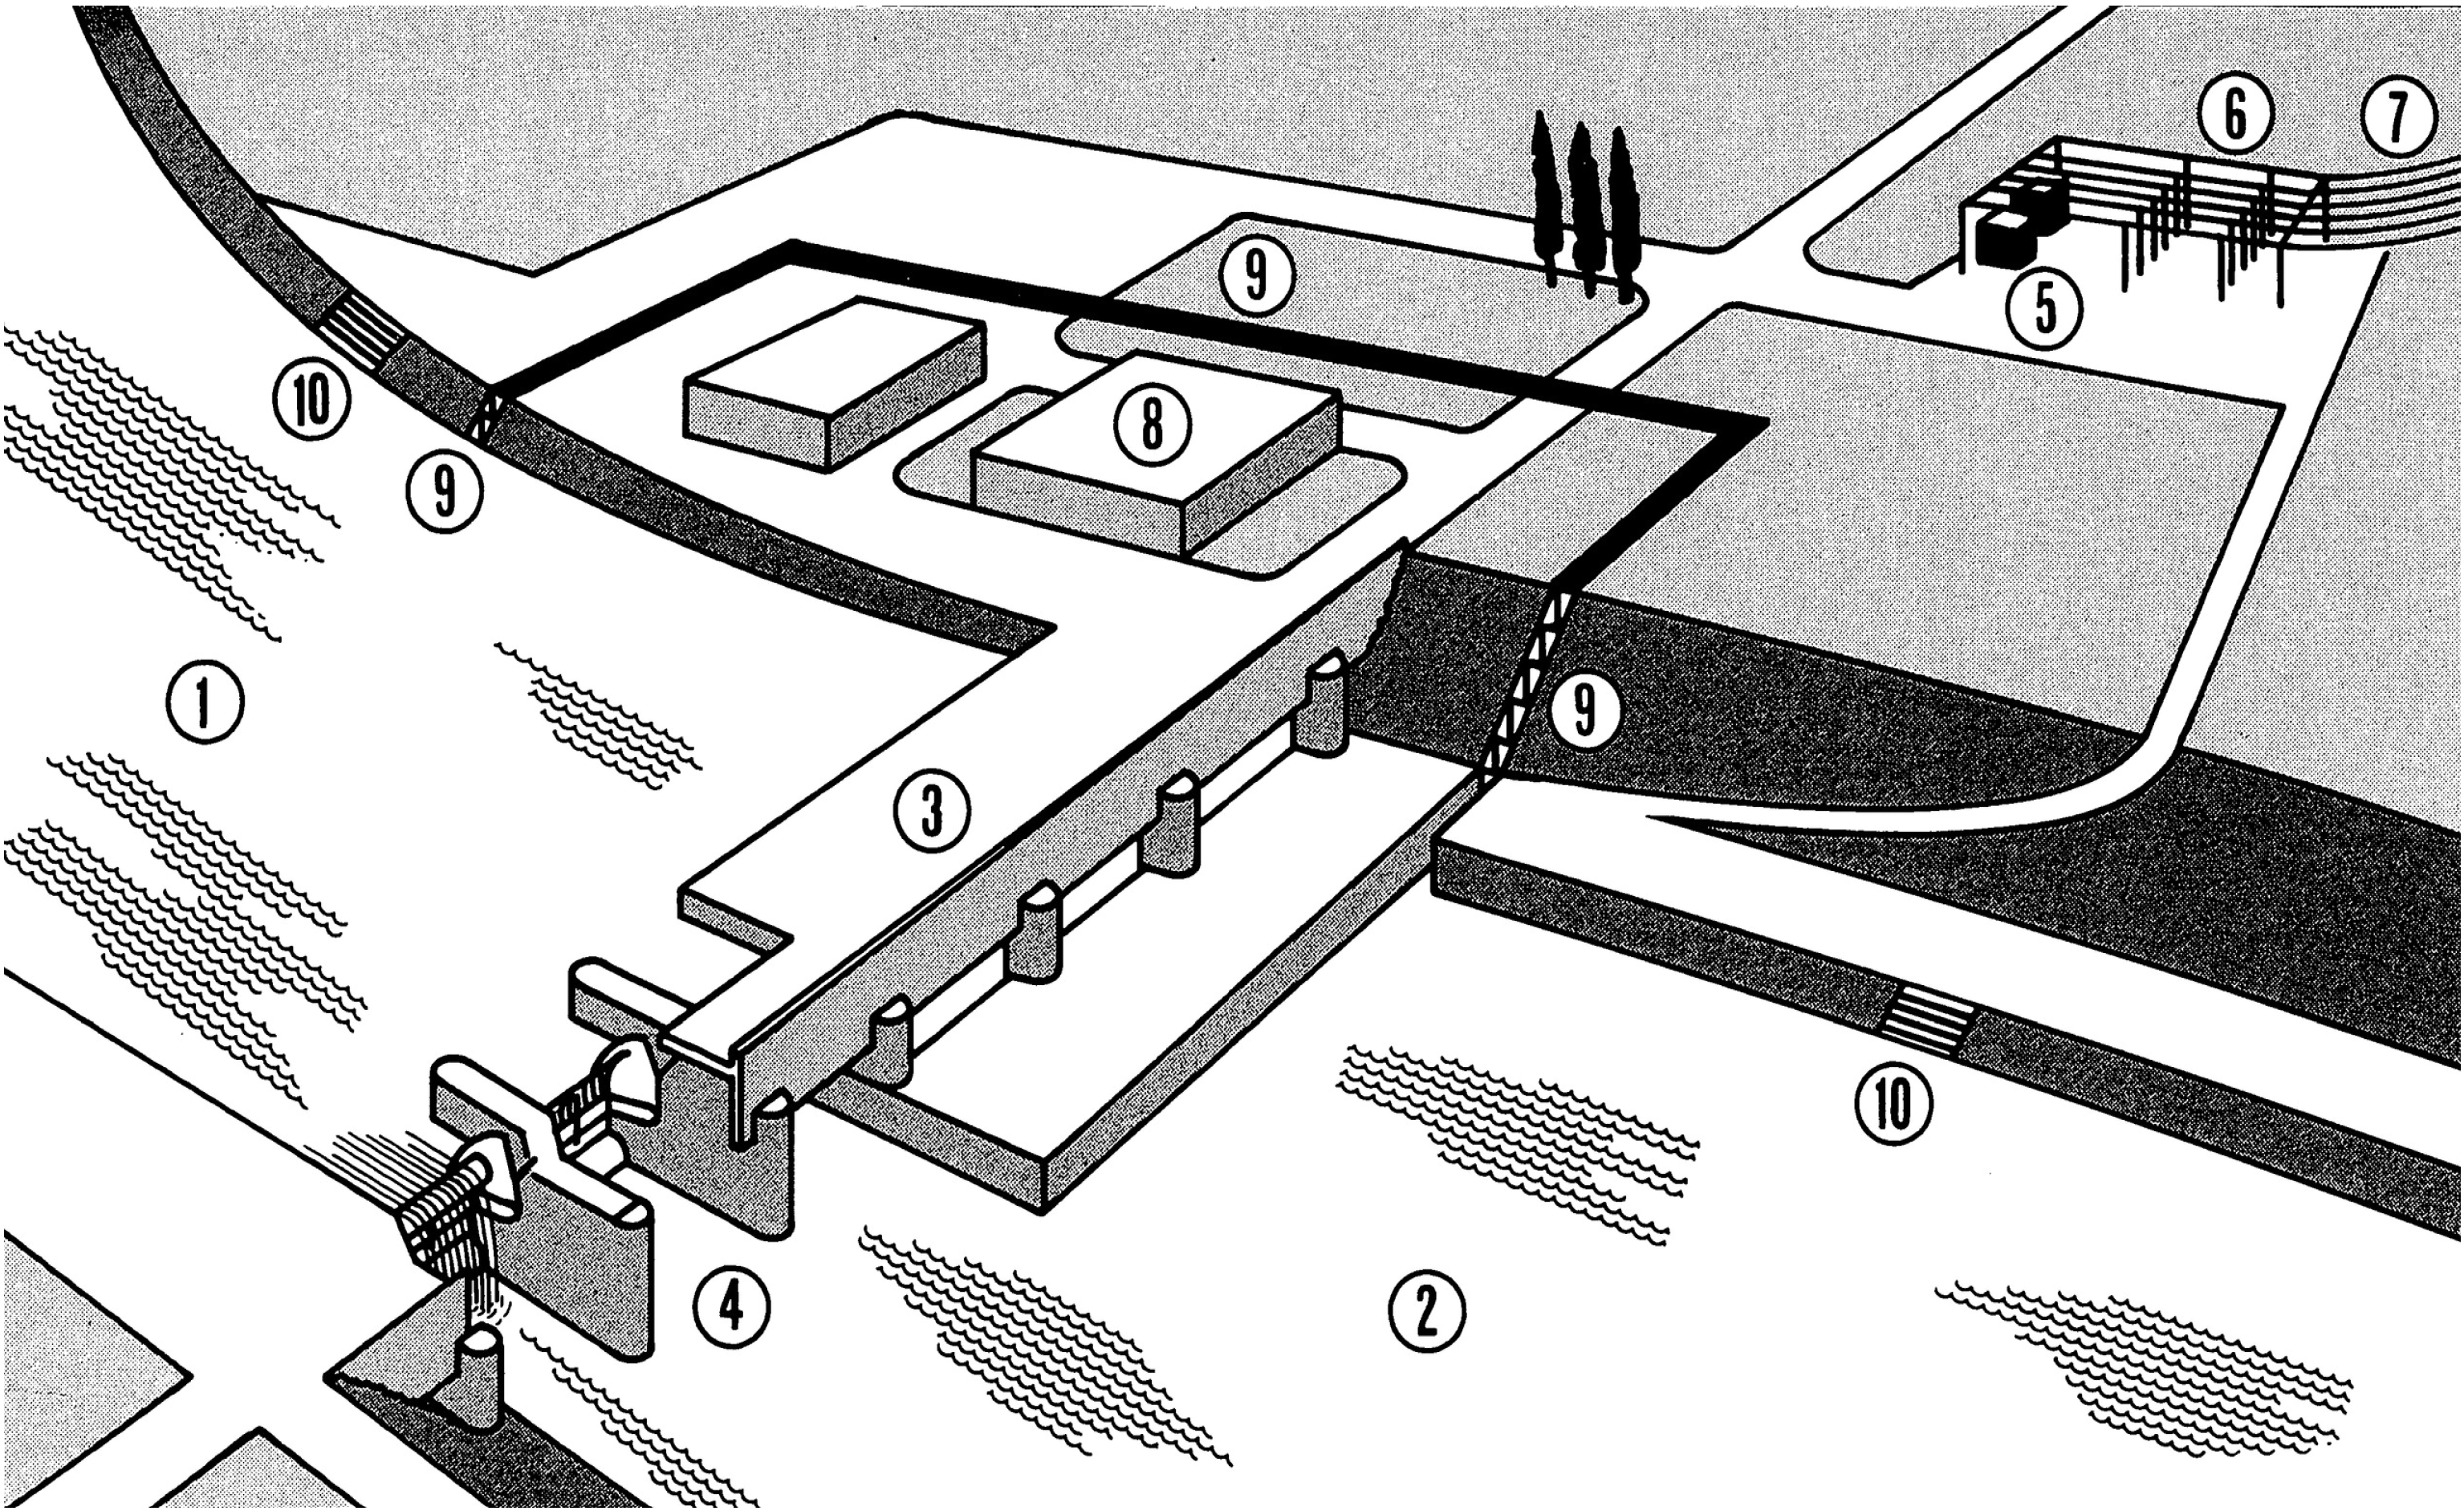
\includegraphics[width=0.95\columnwidth, align=c]{images/Laufwasserkraftwerke.png}
\end{center}

\begin{minipage}[c]{0.38\columnwidth}
    \begin{tabular}{c l}
        1 & Oberwasser \\ 
        2 & Unterwasser \\ 
        3 & Maschinenhaus \\
        4 & Stauwehr \\
        5 & Transformatoren \\
    \end{tabular}
\end{minipage}
\hfill
\begin{minipage}[c]{0.58\columnwidth}
    \begin{tabular}{c l}
        6 & Schaltanlage \\
        7 & Leitungen \\
        8 & Betriebsgebäude \\
        9 & Fischtreppe \\
        10 & Einrichtung für den Schiffstransport \\
    \end{tabular}
\end{minipage}



\subsection{LWK mit Kaplanturbinen Vertikal}

\begin{center}
    \includegraphics[width=0.95\columnwidth, align=c]{images/Laufwasserkraftwerke_Kaplanturbine_Vertikal.png}
\end{center}

\begin{minipage}[t]{0.38\columnwidth}
    \begin{tabular}{c l}
        1 & Oberwasser \\
        2 & Unterwasser \\
        3 & Rechen \\
        4 & Spirale \\
        5 & Stützschaufeln \\
        6 & Leitschaufeln \\
        7 & Laufrad \\
        8 & Laufradschaufeln \\
        9 & Saugrohr \\
    \end{tabular}
\end{minipage}
\hfill
\begin{minipage}[t]{0.58\columnwidth}
    \begin{tabular}{c l}
        10 & Generator \\
        11 & Maschinenhaus \\
        12 & Rechenreinigungsmaschine \\
        13 & Geschwemmselrinne \\
        14 & Zangengreifer \\
        15 & Dammbalken \\
        16 & Nuten für Dammbalken \\
        17 & Dammbalkenkran \\
           &  \\
    \end{tabular}
\end{minipage}



\subsection{LWK mit Kaplanturbinen Horizontal}

\begin{center}
    \includegraphics[width=0.95\columnwidth, align=c]{images/Laufwasserkraftwerke_Kaplanturbine_Horizontal.png}
\end{center}

\begin{minipage}[t]{0.38\columnwidth}
    \begin{tabular}{c l}
        1 & Oberwasser \\
        2 & Unterwasser \\
        3 & Rechen \\
        4 & Leitschaufeln \\
        5 & Laufrad \\
        6 & Laufradschaufeln \\
        7 & Turbinenwelle \\
        8 & Generator \\
        9 & Gehäuse \\
    \end{tabular}
\end{minipage}
\hfill
\begin{minipage}[t]{0.58\columnwidth}
    \begin{tabular}{c l}
        10 & Sockel \\
        11 & Einstiegsschächte \\
        12 & Maschinenhalle \\
        13 & Rechenreinigungsmaschine \\
        14 & Geschwemmselrinne \\
        15 & Zangengreifer \\
        16 & Dammbalken \\
        17 & Nuten für die Dammbalken \\
        18 & Dammbalkenkran \\
    \end{tabular}
\end{minipage}





































        %\newpage
\section{Turbinen Kenngrössen}
\subsection{Nettofallhöhe und Durchfluss}

\subsection{Hydraulische Leistung}

$\boxed{P_{\text{hyd}} = \rho \cdot Q \cdot g \cdot H_n}$

\renewcommand{\arraystretch}{1.2} % Erhöht Zeilenhöhe für bessere Lesbarkeit
\begin{tabular}{@{} l p {7cm} l @{}}
    $[P_{\text{hyd}}]$  & Hydraulische Leistung \dotfill & $W$ \\
    $[Q]$               & Nutzwassermenge \dotfill & $m^3/s$ \\
    $[H_n]$             & Nettofallhöhe \dotfill & $m$ \\
    $[\rho]$            & Dichte des Wassers ($\rho = 1000$) \dotfill & $\frac{kg}{m^3}$ \\
    $[g]$               & Erdbeschleunigung ($g = 9.81$) \dotfill & $\frac{m}{s^2}$ \\
\end{tabular}




\subsection{Mechanische Leistung an der Turbinenwelle}

$\boxed{P_{\text{mech}} = \omega \cdot M}$

\renewcommand{\arraystretch}{1.2} % Erhöht Zeilenhöhe für bessere Lesbarkeit
\begin{tabular}{@{} l p {6cm} l @{}}
    $[P_{\text{mech}}]$  & Mechanische Leistung   \dotfill & $W$ \\
    $[\omega]$           & Winkelgeschwindigkeit \dotfill & $\frac{\text{rad}}{s}$ \\
    $[M]$                & Drehmoment            \dotfill & $Nm$ \\
\end{tabular}


\subsection{Winkelgeschwindigkeit}

$\boxed{\omega = 2 \cdot \pi \cdot n}$

\renewcommand{\arraystretch}{1.2} % Erhöht Zeilenhöhe für bessere Lesbarkeit
\begin{tabular}{@{} l p {6cm} l @{}}
    $[\omega]$  & Winkelgeschwindigkeit \dotfill & $\frac{\text{rad}}{s}$ \\
    $[n]$       & Drehzahl              \dotfill & $\frac{1}{s}$ \\
\end{tabular}


\subsection{Betriebszustände der Maschinengruppe}
\textbf{(Maschinengruppe = Turbine/Pumpe + Generator/Motor)}

\begin{itemize}
    \item Inselbetrieb
    \item Parallelbetrieb, Verbundbetrieb
    \item Instationäre Vorgänge
    \begin{itemize}
        \item Anfahren und Abstellen
        \item Lastabwurf $\Rightarrow$ Überdrehzahl
    \end{itemize}
\end{itemize}

\textbf{Durchgangsdrehzahl $n_D$} (auch Schleuderdrehzahl genannt) $\Rightarrow$ höchste erreichbare Drehzahl ohne Last (z.B. bei Versagen des Generators)

Die Durchgangsdrehzahl ist eine Bemessungsgröße. Die Maschinengruppe darf bei der Durchgangsdrehzahl keinen Schaden erleiden.




















        %\input{sections/06_Gasturbinenkraftwerke.tex}
        %\input{sections/07_Gas_und_Dampfturbinenkraftwerke.tex}
        %\input{sections/08_Kombianlagen_für_Kraft-und_Wärmekopplung.tex}
        %\section{Atomkraftwerk}

\subsubsection{Merkmale Nukleare Dampferzeugung}

\begin{outline}
  \1 Leistungsfähige Energiequelle
  \1 CO2 - freie Produktion elektrischer Energie
  \1 Aufwändige Technologie
  \1 Sicherheit
  \1 Tiefenlager radioaktiver Stoffe
  \1 Diskussion in Politik, Gesellschaft, Ethik
\end{outline}


\subsubsection{Kernprozesse für die Energiegewinnung}

\begin{outline}
  \1 Künstliche Kernspaltung schwerer Kerne (Fission)
    \2 → Kernkraftwerke 3. Generation
    \2 (Stand der Technik)
    
  \1 Umwandlung von schweren Kernen in gut spaltbare Kerne im Brutprozess (Konversion)
    \2 → Kernkraftwerke 4. Generation
    \2 (in Entwicklung)
    
  \1 Verschmelzung leichter Kerne zu einem Kern (Fusion)
    \2 → Grundlagenforschung in Bearbeitung
\end{outline}


\subsection{Kernphysikalische Grundlagen}

$\boxed{A = Z + N}$ \quad Nuklid-Schreibweise: $\boxed{\text{\ce{^{A}_{Z}Element}} }$ \quad \text{z.\,B.} \quad \text{\ce{^{235}_{92}U}}

\vspace{1em}
\renewcommand{\arraystretch}{1.2}
\begin{tabular}{@{} l p{6cm} l @{}}
    $[A]$ & Anzahl Kerneteilchen eines Atoms \dotfill & $-$ \\
    $[Z]$ & Anzahl Protonen (Kernladungszahl) \dotfill & $-$ \\
    $[N]$ & Anzahl Neutronen \dotfill & $-$ \\
\end{tabular}



\subsection{Spaltung schwerer Kerne}

\begin{outline}
    \1 Spaltung schwerer Kerne
    \1 Einige Isotope besitzen die Eigenschaft, dass sie beim Beschießen mit langsamen Neutronen diese im Kern absorbieren und in zwei Tochterkerne zerfallen, wobei gleichzeitig 2–3 Neutronen frei werden.

    \vspace{0.2cm}

    $\boxed{
    \ce{^{235}_{92}U + ^{1}_{0}n \rightarrow  ^{89}_{36}Kr + ^{144}_{56}Ba + 3 ^{1}_{0}n + 200MeV}
    }$

    \vspace{0.2cm}

    \1 Bindungsenergie wird dabei frei.\\
        Im Mittel sind dies: 
        \textbf{200 MeV = $\bm{3{,}2 \cdot 10^{-11}}$ Ws pro Spaltung}
    \1 Die „schnellen“ Neutronen müssen abgebremst werden ($\Rightarrow$  thermische Neutronen), so dass der Prozess nicht abbricht.\\
    Dies geschieht mit einem Moderator wie „leichtes“ Wasser oder Graphit.
    \1 Werden genügend thermische Neutronen zur Verfügung gestellt, hält sich durch eine Kettenreaktion der Spaltungsprozess selbst aufrecht.
\end{outline}


\crd{To be continued ...}





















        %\section{Windenergie}


\subsection{Windeleistung}

\includegraphics[width=0.95\columnwidth, align=c]{images/WEK_Leistungs-und_Drehzahlregelung.png}

$
\boxed{
P_{\text{max}} = \frac{dW}{dt} = \frac{A \cdot \rho_{\text{Luft}}}{2} \cdot v_1^3
}
\quad
\boxed{
P_W = c_P \cdot \frac{A \cdot \rho_{\text{Luft}}}{2} \cdot v_1^3
}
$ \quad Achtung! $v_1$ ist hoch 3!


\renewcommand{\arraystretch}{1.2}
\begin{tabular}{@{} l p{8cm} l @{}}
    $[P_{\text{max}}]$ & Theoretische Windleistung \dotfill & $W$ \\
    $[P_W]$            & Effektiv nutzbare praktische Windleistung \dotfill & $W$ \\
    $[c_P]$            & Leistungsbeiwert, $c_P = 0.4 ... 0.5$ \dotfill & $-$ \\
    $[A]$              & Rotorfläche (projizierte Fläche senkrecht zur Strömung) \dotfill & $m^2$ \\
    $[\rho_{\text{Luft}}]$ & Dichte Luft, $\approx 1{,}29 \, \frac{kg}{m^3}$ \dotfill & $\frac{kg}{m^3}$ \\
    $[v_1]$            & Anströmgeschwindigkeit des Windes \dotfill & $\frac{m}{s}$ \\
\end{tabular}



\section{Windenergiekonverter (WEK)}
\subsection{Netzkopplung}

DU = Direktumrichter, ZKU = Zwischenkreis-Umrichter\\

\subsubsection{Direkte Netzkopplung mit ASM}
\includegraphics[width=0.6\columnwidth]{images/Direkte Netzkopplung mit ASM.png}

\subsubsection{Direkte Netzkopplung mit SM}
\includegraphics[width=0.6\columnwidth]{images/Direkte Netzkopplung mit SM.png}

\subsubsection{Direkte Netzkopplung mit ASM und DU im Läufer}
\includegraphics[width=0.6\columnwidth]{images/Direkte Netzkopplung mit ASM und Direktumrichter im Läufer.png}

\subsubsection{Direkte Netzkopplung mit SM über Gleichstromzwischenkreis}
\begin{itemize}
    \item variable Drehzahl
\end{itemize}

\vspace{0.1cm}

\includegraphics[width=0.6\columnwidth]{images/Direkte Netzkopplung mit SM über einen Gleichstromzwischenkreis, variable Drehzahl.png}

\subsubsection{Direkte Netzkopplung mit ASM und ZKU im Läufer}

\begin{itemize}
    \item übersynchrone Strorichter-Kaskade
    \item variable Drehzahl
\end{itemize}

\vspace{0.1cm}

\includegraphics[width=0.6\columnwidth]{images/Direkte Netzkopplung mit ASM und Zwischenkreis-umrichter im Läufer.png}
















        \section{Netze Allgemein}


\subsubsection{Stromnetz früher}

\begin{center}
    \includegraphics[width=0.95\columnwidth, align=c]{images/Aufgabe_des_Netzes_früher.jpg}
\end{center}


\subsubsection{Stromnetz heute}

\begin{center}
    \includegraphics[width=0.95\columnwidth, align=c]{images/Aufgabe_des_Netzes_heute.jpg}
\end{center}

\subsection{Interessen der Erzeuger}

\begin{itemize}
    \item \textbf{Erzeuger}
    \begin{itemize}
        \item Freier Netzzugang
        \item Hohe Verfügbarkeit: produzierte Leistung kann jederzeit abgeführt werden
        \item Geringe Kosten
    \end{itemize}
    \item \textbf{Verbraucher}
    \begin{itemize}
        \item Netzanschluss
        \item Hohe Versorgungssicherheit und -qualität
        \item Geringe Kosten
    \end{itemize}
\end{itemize}


\subsection{Anforderungen an das Stromnetz}

\begin{itemize}
    \item Hohe Verfügbarkeit
    \item Hohe Versorgungsqualität
    \item Sicherheit
    \item Wirtschaftlichkeit
    \item Diskriminierungsfreiheit
    \item Transparenz
\end{itemize}



        \section{Netzebenen}

\begin{center}
    \includegraphics[width=0.95\columnwidth, align=c]{images/Netzebenen_1.png}
\end{center}

\begin{tabular}{>{\bfseries}l l l}
    \toprule
    Spannungsebene & Spannungsbereich & Leistung \\
    \midrule
    Höchstspannung   & 380 kV, 220 kV         & > 300 MVA \\
    Hochspannung     & 150 kV bis 50 kV       & < 100 MVA \\
    Mittelspannung   & 36 kV bis 6 kV         & < 30 MVA \\
    Niederspannung   & 0{,}4 kV               & < 1 MVA \\
    \bottomrule
\end{tabular}

\subsection{NE1: Übertragungsnetz}

\begin{itemize}
    \item 380 kV und 220 kV
    \item Zweck
    \begin{itemize}
        \item Abtransport der großen Kraftwerksleistungen (typ. > 300 MVA)
        \item Versorgung der Verteilnetze
        \item Weiträumiger Energietransport
        \item Internationaler Verbundbetrieb, Energieaustausch
    \end{itemize}
    \item \textbf{Ausdehnung:} national, international
    \item \textbf{Topologie:} (stark) vermaschtes Netz
    \item \textbf{Technologie:} fast ausschließlich Freileitungen
\end{itemize}

\subsubsection{Schweizer Stromübertragungsnetz (Daten 2014)}

\begin{center}
    \includegraphics[width=0.95\columnwidth, align=c]{images/Schweizer_übertragungsnetz.png}
\end{center}

\begin{itemize}
    \item Gesamtlänge Übertragungsnetz Inland: 6700 km
    \begin{itemize}
        \item Länge 380 kV: 1780 km
        \item Länge 220 kV: 4920 km
    \end{itemize}
    
    \item Gesamtzahl Leitungen im Übertragungsnetz: 246
    \begin{itemize}
        \item Leitungen 380 kV: 48
        \item Leitungen 220 kV: 198
    \end{itemize}
    
    \item Anzahl Netzübergänge in das Ausland: 41
\end{itemize}

\subsubsection{Entso-E}

\begin{center}
    \includegraphics[width=0.95\columnwidth, align=c]{images/Entso_E.png}
\end{center}

\begin{itemize}
    \item koordinierter Systembetrieb
    \item koordinierte Marktlösungen
    \item koordinierte Systementwicklung
\end{itemize}




\subsection{NE3: Überregionales Verteilnetz}

\begin{itemize}
    \item 150 kV, 132 kV, 60 kV
    \item Zweck
    \begin{itemize}
        \item Abtransport mittlerer Kraftwerksleistungen (typ. 100 MVA)
        \item Anschluss großer Industriekunden
        \item Überregionale Verteilung
    \end{itemize}
    \item Ausdehnung: mehrere Kantone
    \item Topologie: (leicht) vermaschtes Netz oder Ringnetz
    \item Technologie: vorwiegend Freileitungen
\end{itemize}

\subsection{NE5: Verteilnetz}


\begin{itemize}
    \item 20 kV, 10 kV
    \item Zweck
    \begin{itemize}
        \item Abtransport kleiner Kraftwerksleistungen (\(< 30\,\text{MVA}\))
        \item Anschluss von Industrie- und Gewerbekunden
        \item Regionale Verteilung
    \end{itemize}
    \item Ausdehnung: Kanton, Tal
    \item Topologie: Ringnetz, Strahlennetz
    \item Technologie: Freileitungen und Kabel
\end{itemize}

\subsection{NE7: Verteilnetz}

\begin{itemize}
    \item 400 V
    \item Zweck
    \begin{itemize}
        \item Abtransport kleinster Einspeisungen (kVA)
        \item Feinverteilung zum Endverbraucher
        \item Anschluss von Haushaltskunden
    \end{itemize}
    \item Ausdehnung: typ. Gemeinde
    \item Topologie: offener Ring, Strahlennetz
    \item Technologie: Freileitungen und Kabel
\end{itemize}






















        \section{Netztopologien}


\subsection{Strahlnetz}

\includegraphics[width=0.55\columnwidth, align=c]{images/Strahlnetz.png}

\textbf{Pro:}
    \begin{itemize}
        \item geringer Planungsaufwand
        \item große Übersichtlichkeit bei der Fehlersuche
        \item geringe Anforderungen an den Netzschutz
    \end{itemize}
\vspace{1em}
\textbf{Contra:}
    \begin{itemize}
        \item größer werdende Spannungsabfälle mit zunehmendem Abstand von der Einspeisung
        \item höhere Leistungsverluste mit zunehmendem Abstand von der Einspeisung
    \end{itemize}


\subsection{Ringnetz}

\includegraphics[width=0.55\columnwidth, align=c]{images/Ringnetz.png}

\textbf{Pro:}
\begin{itemize}
    \item höhere Versorgungssicherheit
    \item geringere Verluste
    \item verbesserte Spannungshaltung
\end{itemize}

\vspace{1em}
\textbf{Contra:}
\begin{itemize}
    \item höhere Anspruch an die Qualifikation des Wartungspersonals
\end{itemize}

\subsection{Maschennetz}

\includegraphics[width=0.55\columnwidth, align=c]{images/Maschennetz.png}

\textbf{Pro:}
\begin{itemize}
    \item eine optimale Versorgungszuverlässigkeit
    \item optimale Spannungshaltung
    \item minimale Leistungsverluste
\end{itemize}

\vspace{1em}
\textbf{Contra:}
\begin{itemize}
    \item hohe Investitionskosten
    \item hohe Projektions- und Wartungsaufwand
    \item höhere Kurzschlussströme
\end{itemize}














        \newcolumn
\section{Leitungen}

\textbf{Aufgabe:}
\begin{itemize}
    \item  Energieübertragung und -verteilung\\
\end{itemize}

\textbf{Wichtigsten Leitungsarten:}
\begin{itemize}
    \item \textbf{Freileitungen} in praktisch allen Spannungsebenen von der Niederspannung bis zur Höchstspannung.
    \item \textbf{Kabelleitungen} mehr in den unteren Spannungsebenen.
\end{itemize}


\subsection{Freileitungen}
\subsubsection{Freileitungen: Vor- und Nachteile}

\textbf{Pro:}
\begin{itemize}
    \item günstige Investitionskosten
    \item bessere Zugänglichkeit bei Reparaturen $\Rightarrow$ kürzere Wiederinbetriebnahmezeiten
\end{itemize}
\vspace{1em}
\textbf{Contra:}
\begin{itemize}
    \item atmosphärischen Einwirkungen ausgesetzt
    \item Akzeptanzprobleme
\end{itemize}

\begin{itemize}
    \item \textbf{Material:}
    \begin{itemize}
        \item Al-Seile (99{,}5\% Al), Aldrey-Seile (> 98{,}5\% Al, Mg, Si, Fe) und Al-Stahl-Seile\\ 
        (Verhältnis Alu:Stahl typ. 6:1, z.\,B. 240/40 mm\textsuperscript{2}), Kupfer ist bei neuen Leitungen immer seltener
        \item Aluminium-Drähten $\Rightarrow$ eine gute elektrische Leitfähigkeit
        \item Stahlkern $\Rightarrow$ mechanische Festigkeit
        \item Aluminium hat gegenüber Kupfer einen deutlichen Preisvorteil
    \end{itemize}

    \item Ab 220\,kV $\Rightarrow$ Bündelleiter $\Rightarrow$ Sie führen also zur 
    \textbf{Verminderung des Wellenwiderstandes} und damit 
    \textbf{zur Erhöhung der übertragbaren Leistung.}

    \item \textbf{Hochtemperaturleiter:}
    \begin{itemize}
        \item normale Leiterseile $T_{\text{max}} = 80\,^{\circ}\mathrm{C}$
        \item Hochtemperaturseilen $T_{\text{max}} = 210\,^{\circ}\mathrm{C}$
        \item \textbf{Steigerung der Übertragungskapazität um bis zu 50 Prozent}
    \end{itemize}
\end{itemize}

\subsubsection{Masten}

\textbf{Funktionen:}
\begin{itemize}
    \item \textbf{Tragmast:} Tragwerke für die Aufhängung der Leiter einer Freileitung
    \item \textbf{Abspannmasten:} An Winkelpunkten nehmen sie die Zugkräfte der Leiterseile auf.
    \item \textbf{Verdrillmast:} alle Aussenleiter eines Stromkreises auf dem Mast tauschen ihre Plätze\\
    (verbessertes Übertragungsverhalten).
\end{itemize}

\vspace{1em}
\textbf{Materialien:}
\begin{itemize}
    \item Stahl-Gittermast
    \item Betonmast
    \item Stahlrohrmast
    \item Holzmast
\end{itemize}


\subsubsection{Unterscheidungsmerkmale Freileitungen}

\textbf{Die wichtigsten Unterscheidungsmerkmale:}

\begin{itemize}
    \item Anzahl Phasen
    \item Länge der Isolatorenketten (Je höher die Spannung, umso länger sind die Isolatorenketten)
    \item Abstand der Phasen und Höhe der Masten
\end{itemize}

\begin{minipage}[c]{0.48\columnwidth}
    \begin{center}
        \includegraphics[width=0.9\textwidth, align=c]{images/Freileitungen_1.png}
    \end{center}
\end{minipage}
\hfill
\begin{minipage}[c]{0.48\columnwidth}
    \begin{center}
        \includegraphics[width=0.9\textwidth, align=c]{images/Freileitungen_2.png}
    \end{center}
\end{minipage}
\newcolumn
\subsubsection{Mastenformen}

\begin{minipage}[c]{0.4\columnwidth}
    \textbf{Donaumast}
\end{minipage}
\hfill
\begin{minipage}[c]{0.56\columnwidth}
    \textbf{Einebenenmast}
\end{minipage}
\begin{minipage}[c]{0.4\columnwidth}
    Zwei Drehstromkreise bei denen die Leiter jeweils im Dreieck angeordnet sind
\end{minipage}
\hfill
\begin{minipage}[c]{0.56\columnwidth}
    Niedrigen Bauhöhe und eine grössere Trassenbreite
\end{minipage}

\begin{minipage}[c]{0.4\columnwidth}
    \begin{center}
        \includegraphics[height=5cm, align=c]{images/Mastenformen_1.png}
    \end{center}
\end{minipage}
\hfill
\begin{minipage}[c]{0.56\columnwidth}
    \begin{center}
        \includegraphics[height=5cm, align=c]{images/Mastenformen_2.png}
    \end{center}
\end{minipage}

\vspace{0.25cm}

\begin{minipage}[c]{0.5\columnwidth}
    \textbf{Tonnenmast}\\
    Eine geringe Trassenbreite, sind aber höher als vergleichbare Donaumasten

    \includegraphics[height=5cm, align=c]{images/Mastenformen_3.png}    
\end{minipage}



\subsection{Kabelleitungen}

\subsubsection{Material}

\begin{tabular}{>{\bfseries}l l}
    Leiter: & Kupfer oder Aluminium \\
    Isolierung: & öl-imprägniertes Papier oder Kunststoffe wie Polyäthylen (PE), \\
                & vernetztes Polyäthylen (VPE) sowie Polyvinylchlorid (PVC) \\
    Schutzmantel: & Metall \\
\end{tabular}

\subsubsection{Aufbau}

\includegraphics[width=1\linewidth]{images/Kabelaufbau.png}
\begin{multicols}{3}
    \textbf{Gürtelkabel:}\\
    Nichtradiales elektrisches Feld, Verwendung im Nieder- und Mittelspannungsbereich
    \vfill
    \columnbreak
    \textbf{Dreimantel-Kabel:}\\
    Radiales elektrisches Feld, Verwendung im Nieder- und Mittelspannungsbereich
    \vfill\null
    \columnbreak
    \textbf{Einleiterkabel:}\\
    Radiales elektrisches Feld, Verwendung im oberen Mittelspannungs- und im Hochpannungsbereich
\end{multicols}

\subsubsection{Kabel: Vor- und Nachteile}

\textbf{Pro:}
\begin{itemize}
    \item geschützt vor atmosphärischen Einwirkungen $\Rightarrow$ kleinere Ausfallsrate
    \item bessere Akzeptanz
\end{itemize}

\vspace{1em}
\textbf{Contra:}
\begin{itemize}
    \item schwierigere Zugänglichkeit bei Reparaturen $\Rightarrow$ längere Wiederinbetriebnahmezeiten
    \item im Hochspannungsbereich teurer (wirtschaftlich nur für kurze Strecken)
\end{itemize}


\subsubsection{Erdverkabelung in der Schweiz}

\textbf{Erdverkabelung pro Netzebene in der Schweiz}\\
\begin{tabular}{>{\bfseries}l r}
    Netzebene 1 & 8 km \\
    Netzebene 3 & 1'893 km \\
    Netzebene 5 & 30'607 km \\
    Netzebene 7 & 72'852 km \\
\end{tabular}

\newcolumn
        \newpage
\section{Schaltanlagen / Umspannwerke}

\subsection{Aufgabe}

\begin{itemize}
    \item Stromfluss herstellen oder unterbrechen
    \item Betriebsmittel unter Spannung setzen oder spannungslos schalten
    \item Topologie ändern
    \item Strom- und Spannungsmessung
\end{itemize}

\subsection{Aufbau}

\begin{center}
    \includegraphics[width=0.98\columnwidth]{images/Aufbau_Schaltanlagen_1.png}
\end{center}

\begin{enumerate}
    \item Transformatoren
    \item Trennschalter
    \item Erdungsschalter
    \item Strom- und Spannungswandler
    \item Leistungsschalter
    \item Überspannungsableiter
    \item Sammelschiene
    \item Blitzschutzmast
    \item Portal
    \item Relais- und Betriebsgebäude
\end{enumerate}


\subsection{Transformator}

\begin{itemize}
    \item Veränderung der Spannung
    \item Öl zur Isolation und zum Wärmeabtransport
\end{itemize}

\begin{minipage}[c]{0.58\columnwidth}
    \begin{center}
        \includegraphics[width=0.98\textwidth, align=c]{images/Transformator_1.png}
    \end{center}
\end{minipage}
\hfill
\begin{minipage}[c]{0.38\columnwidth}
    \begin{center}
        \includegraphics[width=0.98\textwidth, align=c]{images/Transformator_2.png}
    \end{center}
\end{minipage}


\subsection{Leistungsschalter}



\begin{minipage}[c]{0.28\columnwidth}
    \begin{center}
        \includegraphics[width=0.98\textwidth, align=c]{images/Leistungsschalter.png}
    \end{center}
    
\end{minipage}
\hfill
\begin{minipage}[t]{0.68\columnwidth}
    \begin{itemize}
        \item Schaltet \textbf{Strom}
        \item Ein- und Ausschalten von Leitungen und Anlagenteile
        \item Schaltet im Normalbetrieb und im Fehlerfall\\(Kurzschlussstromunterbrechung)
    \end{itemize}
\end{minipage}


\subsection{Lastschalter}

\begin{itemize}
    \item Schaltet \textbf{Strom}
    \item Kann bis zu ca. 2-fachem Laststrom unterbrechen
\end{itemize}


\subsection{Trennschalter}

\begin{minipage}[c]{0.5\columnwidth}
    \includegraphics[width=0.98\textwidth]{images/Trennschalter.png}    
\end{minipage}

\begin{itemize}
    \item Leitungs- oder Sammelschienentrennschalter
    \item öffnen eines Stromkreises (Trennung einer Anlage von den restlichen Anlagen)
    \item Die Trennschalter schalten \textbf{keinen Strom}.
\end{itemize}


\subsection{Sonstiges}

\begin{minipage}[c]{0.48\columnwidth}
    \subsubsection{Messwandler}
\end{minipage}
\hfill
\begin{minipage}[c]{0.48\columnwidth}
    \subsubsection{Überspannungsableiter}
\end{minipage}

\begin{minipage}[c]{0.48\columnwidth}
    Messung der Spannung und Strom für Erkennung des Betriebszustandes
\end{minipage}
\hfill
\begin{minipage}[c]{0.48\columnwidth}
    Spannungsabhängiger Widerstand, Bei hoher Spannung verringert sich Widerstand schlagartig
\end{minipage}

\vspace{0.15cm}

\begin{minipage}[c]{0.48\columnwidth}
    \begin{center}
        \includegraphics[width=0.98\columnwidth]{images/Messwandler.png}
    \end{center}
\end{minipage}
\hfill
\begin{minipage}[c]{0.48\columnwidth}
    \begin{center}
        \includegraphics[width=0.98\columnwidth]{images/Überspannungsableiter.png}
    \end{center}
\end{minipage}


\subsection{Schaltfelder Aufbau}

\begin{minipage}[c]{0.48\columnwidth}
    \subsubsection{Einfachsammelschiene}
\end{minipage}
\hfill
\begin{minipage}[c]{0.48\columnwidth}
    \subsubsection{Doppelsammelschiene}
\end{minipage}

\begin{minipage}[c]{0.48\columnwidth}
    \begin{itemize}
        \item übersichtliche und billige Lösung
    \end{itemize}
\end{minipage}
\hfill
\begin{minipage}[c]{0.48\columnwidth}
    \begin{itemize}
        \item ein Sammelschienenwechsel eines beliebigen Feldes jederzeit möglich
    \end{itemize}
\end{minipage}

\vspace{0.15cm}

\begin{minipage}[c]{0.48\columnwidth}
    \begin{center}
        \includegraphics[width=0.98\columnwidth]{images/Einfachsammelschiene.png}
    \end{center}
\end{minipage}
\hfill
\begin{minipage}[c]{0.48\columnwidth}
    \begin{center}
        \includegraphics[width=0.98\columnwidth]{images/Doppelsammelschiene.png}
    \end{center}
\end{minipage}

\vspace{0.15cm}

\begin{minipage}[c]{0.48\columnwidth}
    \subsubsection{Sammelschienenkupplung}
\end{minipage}
\hfill
\begin{minipage}[c]{0.48\columnwidth}
    \subsubsection{Umgehungsschiene}
\end{minipage}

\begin{minipage}[c]{0.48\columnwidth}
    \begin{itemize}
        \item Ermöglicht die Parallelschaltung der beiden Sammelschienensysteme und damit den Sammelschienenwechsel des Feldes ohne Betriebsunterbruch
    \end{itemize}
\end{minipage}
\hfill
\begin{minipage}[c]{0.48\columnwidth}
    \begin{itemize}
        \item Bei dieser Schaltung ersetzt Reserveschalter den Kuppelschalter beim
        Sammelschienenwechsel
    \end{itemize}
\end{minipage}

\vspace{0.15cm}

\begin{minipage}[c]{0.48\columnwidth}
    \begin{center}
        \includegraphics[width=0.98\columnwidth]{images/Sammelscheinenkupplung.png}
    \end{center}
\end{minipage}
\hfill
\begin{minipage}[c]{0.48\columnwidth}
    \begin{center}
        \includegraphics[width=0.98\columnwidth]{images/Umgehungsschiene.png}
    \end{center}
\end{minipage}

\subsection{Reglen beim Schalten (Reihenfolge)}

\subsubsection{Allgemein}
Es muss immer beidseitig Spannungsfrei sein, um ein Teil auszutauschen.\\
Es darf kein Strom fliessen.

\subsubsection{Ausschalten}
Beim Ausschalten werden Leistungsschalter zuerst geöffnet, dann Last- und Trennschalter
\subsubsection{Einschalten}
Beim Einschalten müssen zuerst Trennschalter, dann Lastschalter und zuletzt Leistungsschalter geschlossen werden







       
    \end{layout}
\end{document}
